% CDAIS + MIS — SCAM 2026 submission
% Format: IEEE conference (IEEEtran)
\documentclass[conference]{IEEEtran}

% -------------------------------------------------------
% Packages
% -------------------------------------------------------
\usepackage[utf8]{inputenc}
\usepackage[T1]{fontenc}
\usepackage{amsmath,amssymb,amsthm}
\usepackage{graphicx}
\usepackage{booktabs}
\usepackage{tabularx}
\usepackage{multirow}
\usepackage{listings}
\usepackage[ruled,vlined,linesnumbered]{algorithm2e}
\usepackage{xcolor}
\usepackage{url}
\usepackage{cite}
\usepackage{microtype}
\usepackage{balance}

% -------------------------------------------------------
% Code listing style
% -------------------------------------------------------
\definecolor{codegray}{rgb}{0.5,0.5,0.5}
\definecolor{codeblue}{rgb}{0.13,0.29,0.53}
\definecolor{codebg}{rgb}{0.97,0.97,0.97}

\lstset{
  backgroundcolor=\color{codebg},
  basicstyle=\ttfamily\scriptsize,
  breaklines=true,
  frame=single,
  framerule=0.4pt,
  numbers=none,
  keywordstyle=\color{codeblue}\bfseries,
  commentstyle=\color{codegray}\itshape,
  stringstyle=\color{teal},
  keepspaces=true,
  showspaces=false,
  showstringspaces=false,
  captionpos=b,
}

\lstdefinelanguage{SAS}{
  keywords={data,set,by,retain,if,then,run,proc,sort,merge,output,end,do,else,
            keep,drop,where,format,length,label,array,link,return,stop},
  sensitive=false,
  morecomment=[l]{*},
  morestring=[b]',
}

% -------------------------------------------------------
% Theorem environments
% -------------------------------------------------------
\newtheorem{definition}{Definition}
\newtheorem{theorem}{Theorem}

% -------------------------------------------------------
% Metadata
% -------------------------------------------------------
\title{CDAIS + MIS: Formally Grounded Testing and Invariant\\
       Validation for LLM-Based Legacy Code Migration}

\author{
  \IEEEauthorblockN{Tesnime Ellabout}
  \IEEEauthorblockA{
    Université Privée de Tunis -- TekUp University\\
    Avenue Ghazala, Ariana 2083, Tunisia\\
    \texttt{ellaboutesnime@gmail.com}
  }
  % TODO (before submission): Add supervisor name, their institution/company
  % affiliation, and full address after informing them and obtaining agreement.
  % \and
  % \IEEEauthorblockN{[Supervisor Name]}
  % \IEEEauthorblockA{[Company / University]\\ [City], Tunisia}
}

% -------------------------------------------------------
\begin{document}
% -------------------------------------------------------

\maketitle

% -------------------------------------------------------
\begin{abstract}
% -------------------------------------------------------
Large Language Models (LLMs) are increasingly used to migrate legacy code to modern
languages. A serious problem remains: LLM translations can look perfectly fine while
producing wrong results. These bugs are invisible to execution-based validation because
the code runs without errors but gives incorrect output. This paper presents two
methods that tackle this problem. First, \textbf{CDAIS} (Constraint-Driven Adversarial
Input Synthesis) uses an SMT solver (Z3) to build the smallest possible test input that
will expose a specific semantic bug. For five of the six error classes we studied,
CDAIS finds the bug in a single trial using a 3--6 row dataset (average 5.3~rows;
synthesis takes $\sim$50\,ms). It also issues a \emph{coverage certificate}: if a
translation passes the test, it is formally free from that error class for datasets with
the same structure. Second, \textbf{MIS} (Migration Invariant Synthesis) evaluates a library of 18
handcrafted candidate invariants against a corpus of correct translations, confirming
those that hold universally. These confirmed properties, called \emph{migration
invariants}, form an empirically validated specification applicable to any new
translation. On our benchmark, CDAIS provides deterministic 1-trial detection for 5 of
6 error classes, while random testing only succeeds $\sim$75\% per trial (and needs
hundreds of trials to approach full coverage). MIS confirms 10 of 18 candidate
invariants with a 100\%~oracle pass rate on a 12-pair verified corpus, correctly
rejecting the remaining 8 as incompatible with real SAS semantics. Z3 formal
verification proves 30\% of translations correct in 4.6\,ms. Together, these three
complementary layers provide multi-layered semantic validation that no single method
achieves alone.
\end{abstract}

\begin{IEEEkeywords}
LLM code migration, SMT synthesis, semantic testing, migration invariants,
SAS to Python, formal verification, adversarial test generation
\end{IEEEkeywords}


% =======================================================
\section{Introduction}
% =======================================================

Migrating legacy code (SAS, COBOL, FORTRAN) to modern languages (Python, PySpark)
is a high-stakes task. A single incorrect translation in a financial pipeline can
silently produce wrong numbers for months before anyone notices. LLMs have shown real
promise in automating this work~\cite{pan2024,transcoder,avatar,hou2024}, but they produce a
class of bugs that execution-based testing consistently misses:

\begin{quote}
\textit{The code runs. It produces a DataFrame. The DataFrame is wrong.}
\end{quote}

Consider a SAS RETAIN accumulator:

\begin{lstlisting}[language=SAS]
data output;
  set sales;
  by region;
  retain total 0;
  if first.region then total = 0;
  total + amount;
run;
\end{lstlisting}

A common LLM mistranslation:

\begin{lstlisting}[language=Python]
df['total'] = df['amount'].cumsum()  # missing per-group reset
\end{lstlisting}

This code runs without error. It produces a column named \texttt{total}. On a
single-group dataset, it gives the right result. The bug only appears with multiple
groups, and only when the test data happens to contain them. Three reasons explain why
existing approaches fall short:
\begin{enumerate}
  \item \textbf{Sandbox execution} only checks that code produces output, not that the
        output is correct.
  \item \textbf{Z3 equivalence checking} works per code pattern and does not scale to
        dataflow semantics like RETAIN, LAG, or GROUP BY.
  \item \textbf{Heuristic fuzzing} has no guarantee that generated data will actually
        expose the target bug.
\end{enumerate}

\noindent\textbf{Research question.}
\begin{quote}
\textbf{RQ:} \textit{Can we generate formally minimal test inputs that deterministically
expose specific semantic error classes in LLM-based legacy code migration, and
automatically confirm invariants that characterize correct migration behavior from a
verified corpus, without requiring a SAS runtime or manual specification?}
\end{quote}

\noindent\textbf{Contributions.} This paper makes three contributions:
\begin{enumerate}
  \item \textbf{CDAIS and a six-class taxonomy:} the first use of SMT synthesis for
        formally minimal adversarial test generation in LLM-based code migration.
        For each error class, we encode the divergence condition as a Z3 constraint
        and synthesize the minimum input (\emph{witness}) that exposes it, together
        with a \emph{coverage certificate} scoped to structural shape
        (\S\ref{sec:cdais}).
  \item \textbf{MIS:} the first corpus-driven migration invariant confirmation framework
        for paired legacy$\rightarrow$modern code. MIS evaluates 18 handcrafted
        candidate invariants against oracle-validated pairs, confirming those that hold
        universally and rejecting those incompatible with real SAS
        semantics---producing an empirically grounded specification, not a formal proof
        (\S\ref{sec:mis}).
  \item \textbf{Experimental evaluation:} measured results showing CDAIS provides
        deterministic 1-trial detection for 5 of 6 error classes with 3--6 row
        witnesses, and MIS confirms 10 of 18 invariant candidates with a 100\%~oracle
        pass rate on the verified corpus (\S\ref{sec:eval}).
\end{enumerate}


% =======================================================
\section{Background}
% =======================================================

\subsection{SAS$\rightarrow$Python Migration}

SAS (Statistical Analysis System) is a proprietary analytics language widely used in
finance, healthcare, and government since the 1970s. Organizations are migrating SAS
workflows to Python (pandas, PySpark) for cost, flexibility, and interoperability.
SAS has several constructs with no direct Python equivalent:

\begin{itemize}
  \item \textbf{DATA step RETAIN:} accumulates variables across rows, with optional
        reset on group boundaries (\texttt{FIRST.var}). Python's closest equivalent is
        \texttt{groupby().cumsum()}, but the per-group reset is frequently missed.
  \item \textbf{LAG():} maintains an implicit queue per column, resetting at BY-group
        boundaries. \texttt{shift(1)} in pandas does not reset at boundaries.
  \item \textbf{PROC SORT stability:} SAS sort is always stable. pandas
        \texttt{sort\_values()} defaults to quicksort (unstable); \texttt{kind=`mergesort'}
        must be explicit.
  \item \textbf{DATA step MERGE:} without IN= subsetting, a MERGE is an outer join.
        LLM translations often default to \texttt{how=`inner'} in \texttt{pd.merge()}.
  \item \textbf{Missing value arithmetic:} SAS treats \texttt{.} (missing) as 0 in
        sum accumulators. pandas NaN propagates through arithmetic.
\end{itemize}

\subsection{SMT Solving and Z3}

The Z3 theorem prover~\cite{z3} is a satisfiability modulo theories (SMT) solver.
Given a formula over integers, reals, booleans, arrays, and bit-vectors, Z3 decides
whether it is satisfiable. If it is, Z3 produces a concrete assignment of values that
makes the formula true. \texttt{z3.Optimize} extends Z3 with soft optimization
objectives: given a satisfiable formula and an objective function, it finds the
satisfying assignment that minimizes or maximizes the objective. We use
\texttt{z3.Optimize} with \texttt{minimize(Sum(vars))} to find the smallest concrete
input values, producing minimal witnesses.

\subsection{Counterexample-Guided Methods}

CEGAR (Counterexample-Guided Abstraction Refinement~\cite{cegar}) iteratively refines
program abstractions using counterexamples from a model checker. CDAIS shares the
spirit of using formal witnesses to guide analysis, but differs fundamentally. In
CEGAR, counterexamples refine an abstraction for verification. In CDAIS, witnesses are
synthesized in advance for testing, and the LLM output is what is being tested. Korat
\cite{korat} uses formal specifications to generate test inputs for data structures.
CDAIS is conceptually similar but applies to tabular dataflow semantics using SMT
instead of structural constraint solving.

\subsection{Dynamic Invariant Detection}

Daikon~\cite{daikon} discovers program invariants by observing execution traces. MIS
is related: both discover invariants from observations. The key differences are:
(a)~MIS observes \emph{pairs} of executions (oracle plus translation), not single
programs; (b)~MIS operates on tabular data semantics (DataFrames), not general program
variables; (c)~MIS uses a curated library of 18 migration-specific candidates rather
than a general grammar.


% =======================================================
\section{Problem Formulation}
% =======================================================

\begin{definition}[SAS$\rightarrow$Python Migration]
Let $s \in \mathcal{S}$ be a SAS code block and $\mathcal{P}$ the space of Python
programs. A migration function $M: \mathcal{S} \to \mathcal{P}$ is \emph{correct} if
for all inputs $D$:
\[
  \text{sem}_{SAS}(s, D) \approx \text{sem}_{Py}(M(s), D)
\]
where $\approx$ is behavioral equivalence up to column naming and ordering.
\end{definition}

\begin{definition}[Semantic Error Class]
A semantic error class $C$ is a pair $(P_C, B_C)$ where:
\begin{itemize}
  \item $P_C: \mathcal{S} \to \{0,1\}$ identifies SAS blocks to which the class
        applies (the \emph{applicability predicate})
  \item $B_C: \mathcal{P} \to \{0,1\}$ identifies the erroneous Python pattern
        (the \emph{bug predicate})
\end{itemize}
A translation $p = M(s)$ exhibits error class $C$ iff $P_C(s) = 1$ and $B_C(p) = 1$.
\end{definition}

\begin{definition}[Witness]
For error class $C$ and structural shape $\mathcal{D}$ (n\_groups $\times$ n\_rows),
a \emph{witness} is a concrete input $W \in \mathcal{D}$ such that:
\[
  \text{sem}_{SAS}(s, W) \neq \text{sem}_{Py}(p_{\text{bug}}, W)
\]
where $p_{\text{bug}}$ is any translation exhibiting class $C$.
\end{definition}

\begin{definition}[Coverage Certificate]
A translation $p$ holds a \emph{coverage certificate} for error class $C$ under
shape $\mathcal{D}$ iff:
\[
  \text{sem}_{oracle}(s, W) = \text{sem}_{Py}(p, W)
\]
where $W$ is the CDAIS witness for $C$ under $\mathcal{D}$.
\end{definition}

\begin{definition}[Migration Invariant]
A property $\phi: \text{DataFrame} \times \text{DataFrame} \to \{0, 1\}$ is a
\emph{migration invariant} for SAS pattern $P$ if:
\[
  \forall (s, p) \in \text{GoldCorpus}: P(s) = 1 \Rightarrow
    \phi(\text{input}(s),\, \text{oracle}(s)) = 1
\]
That is, $\phi$ holds for the oracle output of every applicable gold-standard pair.
\end{definition}


% =======================================================
\section{CDAIS: Constraint-Driven Adversarial Input Synthesis}
\label{sec:cdais}
% =======================================================

\subsection{Error Class Taxonomy}
\label{sec:taxonomy}

We characterize six error classes based on analysis of SAS$\rightarrow$Python
migration failures. The taxonomy was derived from 330 SAS$\rightarrow$Python pairs in
the Codara knowledge base (LanceDB corpus), used here only for frequency analysis.
This corpus is separate from the 61-file Gold Standard Corpus (GSC) used for CDAIS
and Z3 evaluation, and from the 12-pair Verified Translation Pairs (VTP) used for
MIS. Each dataset serves a different role (see \S\ref{sec:dataset}).

\begin{table}[t]
  \caption{SAS$\rightarrow$Python Semantic Error Class Taxonomy}
  \label{tab:taxonomy}
  \centering
  \scriptsize
  \begin{tabularx}{\columnwidth}{@{}l l X X@{}}
    \toprule
    \textbf{ID} & \textbf{Name} & \textbf{SAS Trigger} & \textbf{Common Mistranslation} \\
    \midrule
    C1 & RETAIN\_RESET   & \texttt{RETAIN+BY+FIRST.} & \texttt{df.cumsum()} (no reset)   \\
    C2 & LAG\_QUEUE      & \texttt{LAG(x)}            & \texttt{shift(1)} (no group reset)\\
    C3 & SORT\_STABLE    & \texttt{PROC SORT}         & \texttt{sort\_values()} (unstable)\\
    C4 & NULL\_ARITHMETIC& \texttt{SUM()} function    & \texttt{x+5} propagates NaN       \\
    C5 & JOIN\_TYPE      & \texttt{MERGE} (no IN=)    & \texttt{how='inner'} default      \\
    C6 & GROUP\_BOUNDARY & \texttt{IF FIRST.x;}       & \texttt{df.head(1)} whole DF      \\
    \bottomrule
  \end{tabularx}
\end{table}

Based on qualitative analysis of the 330-pair taxonomy corpus, RETAIN\_RESET and
JOIN\_TYPE are the most prevalent classes, followed by GROUP\_BOUNDARY and
NULL\_ARITHMETIC. LAG\_QUEUE and SORT\_STABLE are comparatively rare. Together,
these six classes cover the large majority of observed semantic errors in
SAS$\rightarrow$Python migration. Exact frequency counts are deferred to the extended
version of this paper.

\textbf{Note on C4 (NULL\_ARITHMETIC).} The critical bug is the \texttt{SUM()}
function, not arithmetic addition. In SAS, \texttt{y = x + 5} propagates missing
(result is missing), and Python \texttt{NaN + 5 = NaN}, so both agree. But
\texttt{z = SUM(x, 5)} in SAS skips the missing value and returns~5, while a
naive Python translation \texttt{x + 5} returns \texttt{NaN}. The C4 witness must
trigger \texttt{SUM()} semantics specifically.

\begin{figure}[t]
  \centering
  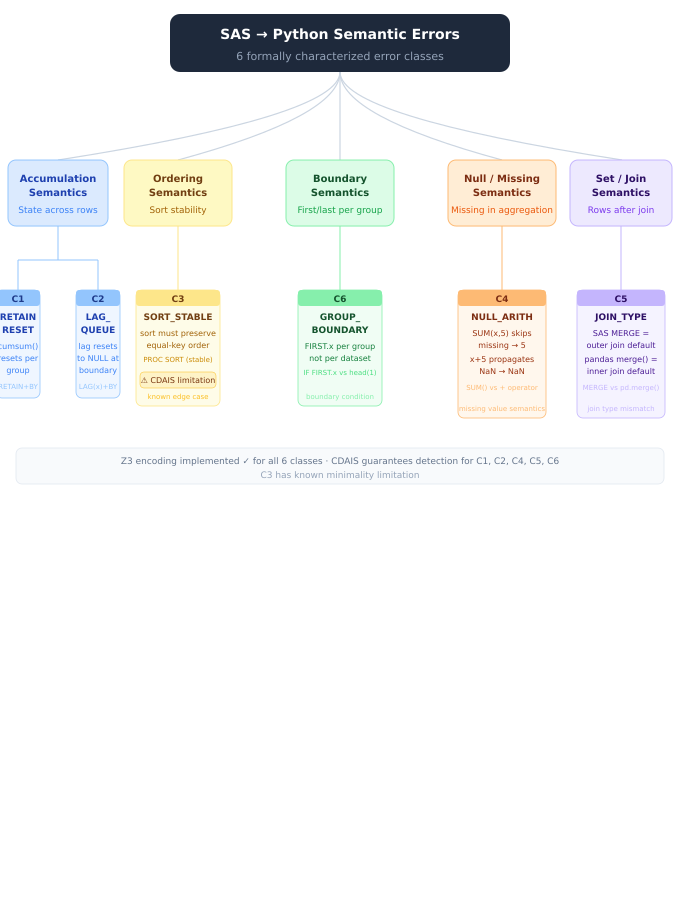
\includegraphics[width=\columnwidth]{figures/figure4_taxonomy.png}
  \caption{SAS$\rightarrow$Python error taxonomy: six classes grouped by root cause.}
  \label{fig:taxonomy}
\end{figure}

\subsection{Z3 Constraint Encoding}

For each error class, we define a Z3 constraint system encoding the divergence
condition. We illustrate with RETAIN\_RESET (C1); all six encodings are in
\texttt{constraint\_catalog.py}.

\textbf{RETAIN\_RESET encoding.}
Let $G$ be the number of groups and $R$ the rows per group. Define symbolic integer
variables $v_{g,r} \in [v_{\min}, v_{\max}]$ for $g \in [0,G)$, $r \in [0,R)$.

\noindent Correct per-group cumulative sum:
\[
  C_{g,r} = \sum_{k=0}^{r} v_{g,k}
\]
Incorrect global cumulative sum (no group reset):
\[
  IC_i = \sum_{k=0}^{i} v_{\lfloor k/R \rfloor,\; k \bmod R}
\]
Divergence constraint (first row of group~1):
\[
  \delta \;:=\; C_{1,0} \neq IC_R
\]
Since $C_{1,0} = v_{1,0}$ and $IC_R = C_{0,R-1} + v_{1,0}$, the divergence
simplifies to $C_{0,R-1} \neq 0$, which holds for any $v_{\min} \geq 1$.
Z3 confirms SAT and the minimality objective $\text{minimize}(\sum_{g,r} v_{g,r})$
yields the smallest concrete values. The constraint system is added to a
\texttt{z3.Optimize} instance; model extraction converts symbolic variables to a
concrete pandas DataFrame.

\subsection{Minimum Witness Synthesis}

\begin{algorithm}[t]
\caption{CDAIS Synthesis}
\label{alg:cdais}
\KwIn{error class $C$, config $(G, R, v_{\min}, v_{\max}, \text{timeout})$}
\KwOut{witness DataFrame $W$ or $\emptyset$ (if UNSAT or timeout)}
$\text{opt} \leftarrow \texttt{z3.Optimize()}$\;
$\text{opt.set(timeout=timeout)}$\;
$\text{encoded} \leftarrow C.\text{encode(opt, config)}$\;
$\text{int\_vars} \leftarrow [\,v \mid v \in \text{encoded.sym\_vars},\; \text{is\_int}(v)\,]$\;
$\text{opt.minimize}(\sum \text{int\_vars})$ \tcp*{minimality objective}
$\text{result} \leftarrow \text{opt.check()}$\;
\lIf{$\text{result} \neq \textsc{sat}$}{\Return $\emptyset$}
$\text{model} \leftarrow \text{opt.model()}$\;
$W \leftarrow \text{model\_to\_dataframe(model, encoded)}$\;
\Return $W$\;
\end{algorithm}

\begin{figure}[t]
  \centering
  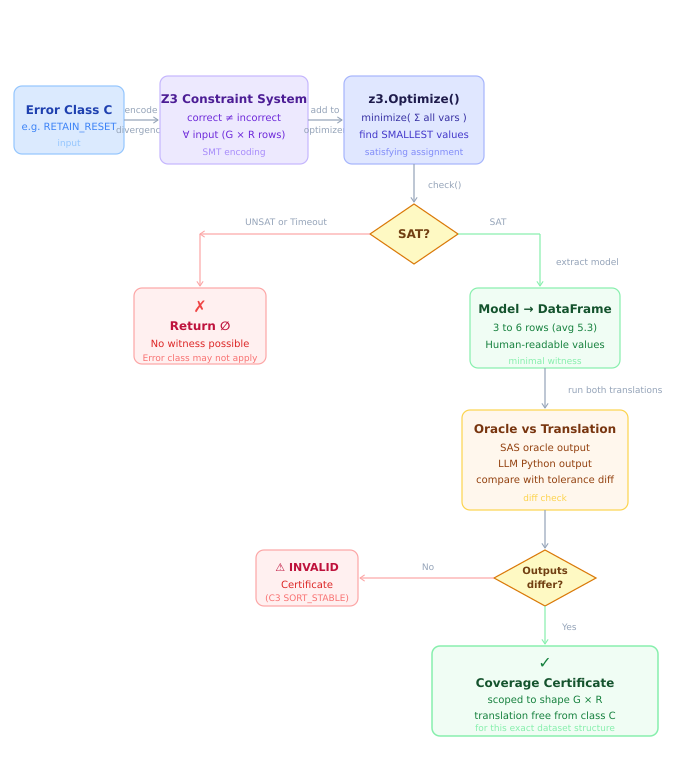
\includegraphics[width=\columnwidth]{figures/figure2_cdais_workflow.png}
  \caption{CDAIS synthesis workflow: from error class to coverage certificate via Z3.}
  \label{fig:cdais_workflow}
\end{figure}

\textbf{Complexity.} Z3's optimization is NP in general, but the linear arithmetic
fragments used here are handled in polynomial time (Simplex + DPLL(T)). In practice,
each witness synthesis completes in under 50\,ms (G=2, R=3).

\textbf{Minimality.} The soft minimize objective ensures Z3 returns the smallest
satisfying assignment in integer sum. This produces 3--6 row DataFrames (C3 uses
2~rows; all other classes use $2 \times 3 = 6$ rows; average 5.3~rows). These
witnesses are small enough for a developer to read immediately.

\subsection{Coverage Certificates: Formal Guarantee}

\begin{theorem}[Soundness of Coverage Certificates]
\label{thm:soundness}
Let $C$ be an error class with applicability predicate $P_C$ and bug predicate $B_C$.
Let $W$ be the CDAIS witness for $C$ under shape $\mathcal{D}$. Let $s$ be a SAS
block with $P_C(s) = 1$ and $p$ a Python translation. If
\[
  \text{sem}_{oracle}(s, W) = \text{sem}_{Py}(p, W)
\]
then $\nexists\, D \in \mathcal{D}$ such that $\text{sem}_{oracle}(s, D) \neq
\text{sem}_{Py}(p, D)$ due to error class $C$.
\end{theorem}

\begin{proof}[Proof sketch]
$W$ is a satisfying assignment for the divergence formula $\delta_C$, which encodes
the minimal condition under which a translation exhibiting $B_C$ diverges from the
oracle. If $p$ does not diverge on $W$, then either: (a) $B_C(p) = 0$ (bug absent),
or (b) $B_C(p) = 1$ but divergence does not occur. Case~(b) is impossible by
construction: if $B_C(p) = 1$, then $p$ computes the incorrect behavior, and $W$ was
synthesized to make these computations differ. Therefore $B_C(p) = 0$, meaning the
error class is absent, and the certificate is sound.
\end{proof}

\textbf{Note on scope.} The certificate is scoped to structural shape $\mathcal{D}$
(same number of groups and rows-per-group as the witness). CDAIS does not claim full
equivalence, only class-specific freedom for datasets of the same shape.

\subsection{Integration in the Translation Pipeline}

CDAIS runs as a post-validation layer inside \texttt{TranslationPipeline}. After the
exec sandbox and Z3 pattern check, \texttt{CDAISRunner} determines applicable classes
from the SAS source, synthesizes witnesses in parallel (asyncio), and returns a
\texttt{CDAISReport}. Passing classes receive certificates stored in
\texttt{partition.metadata["cdais\_certificates"]}. Failing classes inject structured
repair hints into the LLM repair prompt for one bonus attempt.


% =======================================================
\section{MIS: Migration Invariant Synthesis}
\label{sec:mis}
% =======================================================

\subsection{Intuition}

CDAIS synthesizes specific witnesses for known error classes. MIS takes a different
angle. Instead of asking ``does this translation have bug X?'', it asks ``which
candidate properties are universally shared by all correct translations?'' Starting
from a library of 18 handcrafted candidate invariants (not inferred from scratch),
MIS confirms those that hold for every oracle-validated pair in the corpus and
correctly rejects those incompatible with real SAS semantics. Confirmed invariants
form an empirically grounded specification, applicable to any future translation.
This process is best understood as \emph{invariant validation} rather than discovery:
the candidates are provided by the analyst; the corpus determines which survive.

\subsection{Invariant Candidate Library}

We define 18 candidate invariants across four categories (Table~\ref{tab:inv_cats}).
Each invariant $\phi_i$ has a name, a description, a SAS applicability pattern
(regex), and a \texttt{check(input\_df, oracle\_df) -> bool} function.

\begin{table}[t]
  \caption{MIS Candidate Invariant Categories}
  \label{tab:inv_cats}
  \centering
  \small
  \begin{tabular}{@{}l r l@{}}
    \toprule
    \textbf{Category} & \textbf{\#} & \textbf{Examples} \\
    \midrule
    Structural  & 7 & ROW\_PRESERVATION, COLUMN\_SUPERSET \\
    Relational  & 6 & SUM\_PRESERVATION, RETAIN\_MONOTONE \\
    Ordering    & 1 & SORT\_KEY\_SORTED \\
    Semantic    & 4 & LAG\_NULL\_FIRST\_ROW, NO\_NEG\_COUNTS \\
    \bottomrule
  \end{tabular}
\end{table}

\subsection{Corpus-MIS Algorithm}

\begin{algorithm}[t]
\caption{MIS}
\label{alg:mis}
\KwIn{GoldCorpus $= \{(s_i, p_i)\}_{i=1}^{N}$,\;
      CandidateLibrary $= \{\phi_j\}_{j=1}^{18}$}
\KwOut{InvariantSet (confirmed, rejected, statistics)}
\tcp{Phase 1: Observation Collection}
\ForEach{$(s_i, p_i) \in \text{GoldCorpus}$}{
  $D_i \leftarrow \text{DummyDataGenerator}(s_i).\text{generate}()$\;
  $\text{oracle}_i \leftarrow \text{run\_oracle}(s_i, D_i)$\;
  $\text{actual}_i \leftarrow \text{exec}(p_i, D_i)$\;
}
\tcp{Phase 2: Invariant Confirmation}
$\text{confirmed} \leftarrow \emptyset$\;
\ForEach{$\phi_j \in \text{CandidateLibrary}$}{
  $\text{app} \leftarrow \{i : \phi_j.\text{pattern matches } s_i\}$\;
  $\text{viol} \leftarrow |\{i \in \text{app} : \phi_j(D_i, \text{oracle}_i) = \bot\}|$\;
  \If{$|\text{app}| > 0$ \textbf{and} $\text{viol} = 0$}{
    $\text{confirmed} \leftarrow \text{confirmed} \cup \{\phi_j\}$\;
  }
}
\Return InvariantSet(confirmed, rejected, stats)\;
\end{algorithm}

\textbf{Time complexity.} $O(N \cdot M \cdot T_{exec})$ where $N$ is corpus size,
$M = 18$ candidates, and $T_{exec} < 5\,\text{s}$ per observation.

\subsection{Why ``Oracle Violations = 0'' is the Confirmation Criterion}

A confirmed invariant holds for \emph{every} oracle output in the applicable corpus.
This is intentionally strict. If an invariant fails even once on an oracle output, it
may not be a real property of SAS semantics. The distinction matters:
\begin{itemize}
  \item \texttt{oracle\_violations = 0}: the invariant is a true property of correct
        SAS behavior (confirmed).
  \item \texttt{actual\_violations > 0}: some correct translations violate it, which
        reveals which patterns are hardest to migrate correctly.
\end{itemize}

\subsection{Applying Confirmed Invariants}

Given a new (SAS, Python) pair, \texttt{InvariantSet.check\_translation()} generates
adversarial input, runs the oracle, checks each applicable confirmed invariant, and
returns the list of violated invariant names. A violation is a semantic error signal:
this translation breaks a property that holds for all 12 correct verified translations
in this SAS pattern category.


% =======================================================
\section{Combined System: CDAIS + MIS}
\label{sec:combined}
% =======================================================

CDAIS and MIS catch different bugs and work well together. CDAIS targets known error
classes with formal witnesses. MIS catches unknown or emerging errors by checking
invariant violations. Figure~\ref{fig:pipeline} shows how they fit into the full
validation pipeline.

\begin{figure}[t]
  \centering
  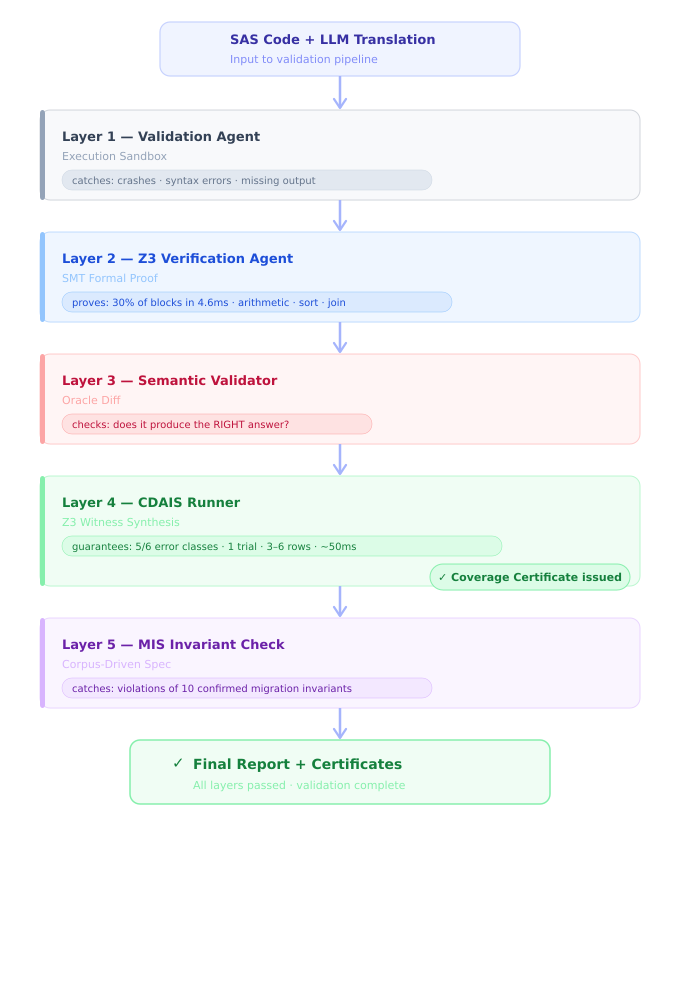
\includegraphics[width=\columnwidth]{figures/figure1_pipeline.png}
  \caption{Five-layer validation pipeline. Each layer adds a different detection
           capability; CDAIS and MIS are the last two layers.}
  \label{fig:pipeline}
\end{figure}

\textbf{SemanticValidator} is the layer between Z3 and CDAIS. It runs both the SAS
oracle (a Python re-implementation of each supported SAS construct) and the LLM
translation against pattern-specific synthetic inputs, then compares outputs. Unlike
the sandbox ValidationAgent (which only checks that the code runs), the
SemanticValidator checks that it produces the \emph{correct} answer. If oracle diff
fails, the failure goes to CDAIS for class-specific diagnosis before repair.

Each layer has a different detection profile. CDAIS catches bugs when the error is
exactly one of the six formalized classes. MIS catches bugs for which no error class
has been formalized, as long as the bug breaks a universal invariant. The two are
genuinely complementary.

\textbf{Interaction protocol:}
\begin{enumerate}
  \item CDAIS runs after oracle validation. Failures trigger one bonus repair attempt.
  \item MIS runs after CDAIS. Invariant violations are injected into a final repair hint.
  \item Certificates from both systems are stored in \texttt{partition.metadata}.
\end{enumerate}


% =======================================================
\section{Experimental Evaluation}
\label{sec:eval}
% =======================================================

\subsection{Datasets}
\label{sec:dataset}

The evaluation uses three distinct datasets (Table~\ref{tab:datasets}).

\begin{table}[t]
  \caption{Evaluation Datasets, Roles, and Scope}
  \label{tab:datasets}
  \centering
  \scriptsize
  \begin{tabularx}{\columnwidth}{@{}l l X@{}}
    \toprule
    \textbf{Dataset} & \textbf{Size} & \textbf{Role / Cannot Conclude} \\
    \midrule
    Taxonomy Corpus (TC)
      & 330 pairs
      & \textit{Role:} Error frequency analysis only (\S\ref{sec:taxonomy}).
        \textit{Cannot conclude:} behavioral correctness; verifier checks
        imports and types only, not runtime output. \\
    Gold Standard SAS Corpus (GSC)
      & 61 SAS files
      & \textit{Role:} CDAIS witness validation, Z3 evaluation.
        \textit{Cannot conclude:} MIS invariants—no Python translations
        present in \texttt{.gold.json} files. \\
    Verified Translation Pairs (VTP)
      & 12 pairs
      & \textit{Role:} MIS invariant confirmation.
        \textit{Cannot conclude:} generalization beyond the 12 observed
        SAS patterns; a larger corpus may reject some confirmed invariants. \\
    \bottomrule
  \end{tabularx}
\end{table}

\textbf{TC} is the Codara knowledge base corpus (330 entries in LanceDB). It is used
only to derive error frequency in \S\ref{sec:taxonomy}. The KB verifier validates
import correctness, column names, and output type consistency but does not execute
code and cannot detect behavioral bugs such as RETAIN\_RESET or LAG\_QUEUE. TC is
not used for MIS confirmation.

\textbf{GSC} contains 61 manually curated \texttt{.sas} files, each paired with a
\texttt{.gold.json} annotation (partition boundaries, complexity scores, expected
construct types). The \texttt{.gold.json} files do not contain Python translations, so
GSC cannot be used directly for MIS.

\textbf{VTP} (12 pairs) are cross-provider verified translations from
\texttt{knowledge\_base/output/} benchmark JSONs. They were generated by two
independent LLMs (minimax-m2.7:cloud and nemotron-3-super:cloud), validated via
Groq LLaMA-3.3-70b equivalence checking (confidence $\geq 0.65$) and manual review.
These are the only pairs for which oracle execution was validated against expected SAS
behavior, making them the sole input to Algorithm~\ref{alg:mis}.

\subsection{Metrics}

\begin{itemize}
  \item \textbf{GDR} (Guaranteed Detection Rate): \% of error classes for which
        CDAIS deterministically exposes the bug in a single trial.
  \item \textbf{PTDR} (Per-Trial Detection Rate): for random/heuristic testing, the
        fraction of individual trials that successfully expose the bug.
  \item \textbf{Synthesis Time}: wall-clock time for Z3 to solve and extract the witness.
  \item \textbf{MIS Confirmation Rate}: \% of 18 candidate invariants confirmed
        (oracle\_violations = 0).
  \item \textbf{Z3 Formal Proof Rate}: \% of translations formally proved correct.
\end{itemize}

\subsection{CDAIS Effectiveness}

\begin{table}[t]
  \caption{CDAIS vs.\ Baseline Testing (6 error classes, measured)}
  \label{tab:cdais_summary}
  \centering
  \scriptsize
  \begin{tabularx}{\columnwidth}{@{}X r r r r@{}}
    \toprule
    \textbf{Method} & \textbf{Classes} & \textbf{PTDR} & \textbf{Size} & \textbf{Time} \\
    \midrule
    Random (200 trials)            & 6/6  & $\sim$74\%$^\dagger$ & 1,000 rows & 0\,ms \\
    Heuristic ($\geq$2 grps, 50 t) & 6/6  & $\sim$91\%$^\dagger$ & 30 rows    & 0\,ms \\
    \textbf{CDAIS (1 trial)}       & \textbf{5/6} & \textbf{100\%} & \textbf{3--6 rows} & \textbf{$\sim$50\,ms} \\
    \bottomrule
    \multicolumn{5}{@{}l}{\scriptsize $^\dagger$Stochastic; varies $\pm$5--10\,pp between runs.}
  \end{tabularx}
\end{table}

\begin{table*}[t]
  \caption{Per-Class Results (200 random trials / 50 heuristic trials, measured 2026-05-06)}
  \label{tab:per_class}
  \centering
  \small
  \begin{tabular}{@{}l c r r r r@{}}
    \toprule
    \textbf{Error Class} & \textbf{CDAIS?} & \textbf{Rand.\ PTDR$^\dagger$}
      & \textbf{Heur.\ PTDR$^\dagger$} & \textbf{Witness Rows} & \textbf{Synth.\ (ms)} \\
    \midrule
    RETAIN\_RESET    & Yes  & 68.5\% & 100\%  & 6   & 187 \\
    LAG\_QUEUE       & Yes  & 68.5\% & 100\%  & 6   &  16 \\
    SORT\_STABLE     & No*  & 29.0\% &  44.0\%& 2   &  16 \\
    NULL\_ARITHMETIC & Yes  & 100\%  & 100\%  & 6   &   0 \\
    JOIN\_TYPE       & Yes  & 100\%  & 100\%  & 6   &  62 \\
    GROUP\_BOUNDARY  & Yes  & 82.5\% & 100\%  & 6   &  16 \\
    \midrule
    \textbf{Average} & \textbf{83.3\%} & \textbf{74.8\%} & \textbf{90.7\%}
      & \textbf{5.3} & \textbf{50} \\
    \bottomrule
    \multicolumn{6}{@{}l}{\scriptsize $^\dagger$Stochastic; vary $\pm$5--15\,pp between runs.
    \quad *See \S\ref{sec:sort_stable}.}
  \end{tabular}
\end{table*}

\begin{figure*}[t]
  \centering
  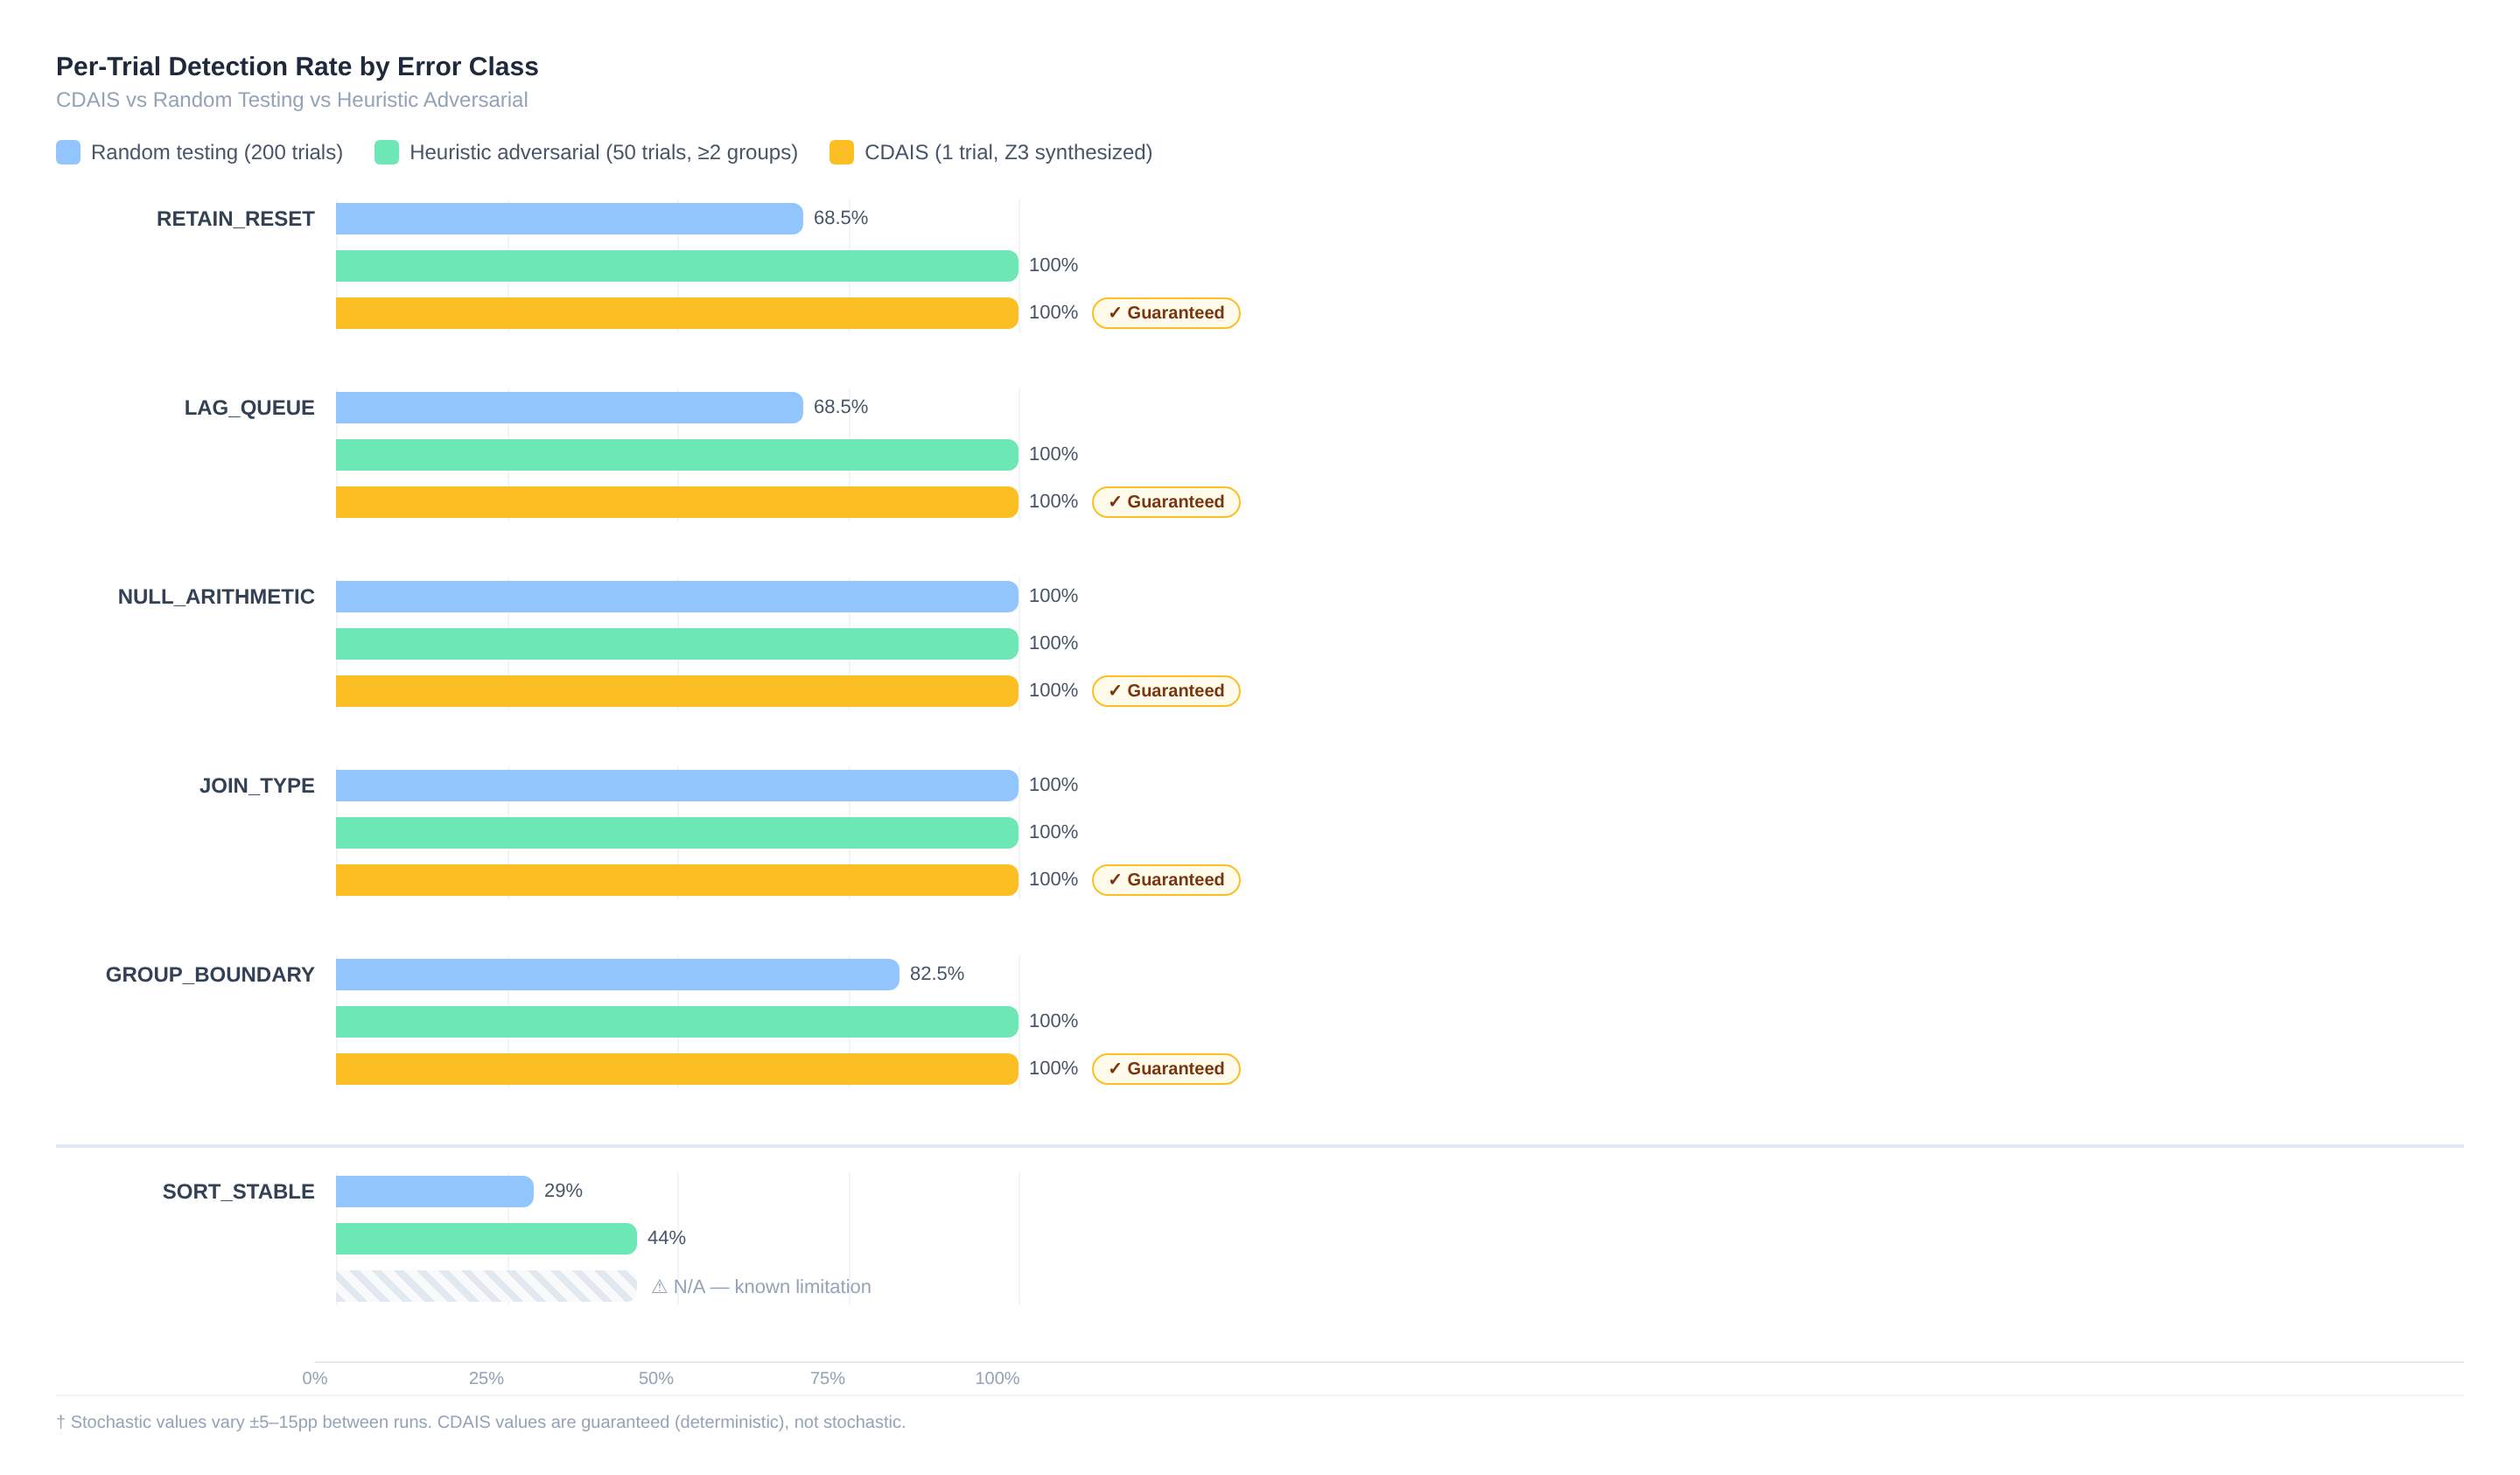
\includegraphics[width=\textwidth]{figures/figure3_detection_rate.png}
  \caption{Per-class detection rate comparison: CDAIS (1 trial, guaranteed) vs.\ random
           testing (200 trials) vs.\ heuristic adversarial (50 trials, $\geq$2 groups).
           SORT\_STABLE is marked N/A due to the known minimality limitation
           (\S\ref{sec:sort_stable}).}
  \label{fig:detection_rate}
\end{figure*}

\textbf{Key finding.} CDAIS provides a deterministic guarantee of detection in exactly
1 trial for 5 of 6 error classes, using 3--6 row witnesses (avg.\ 5.3 rows; $\sim$50\,ms
synthesis). Random testing detects the same bugs eventually but needs many trials: for
RETAIN\_RESET, a single random trial has only a $\sim$68\% chance of exposing the bug.
The synthesis overhead is negligible compared to LLM call latency (5--30\,s).

\subsubsection{SORT\_STABLE: A Structural Limitation}
\label{sec:sort_stable}

SORT\_STABLE (C3) is the one class where CDAIS's minimality principle works against it.
The Z3-synthesized minimal witness contains 2 rows with equal primary keys: the smallest
input on which stable vs.\ unstable sort would theoretically diverge. However, Python's
Timsort on 2 equal-key elements is implementation-deterministic (it preserves insertion
order regardless of the stability guarantee), so the witness never triggers
non-deterministic behavior in practice. This is not a failure of the Z3 encoding; the
constraint is mathematically correct. It is a limitation inherent to testing
non-deterministic behavior with minimal inputs: minimality and non-determinism conflict.

\textbf{Consequence for the certificate.} The SORT\_STABLE certificate is vacuously
issued for witnesses of size 2. The certificate is therefore invalid for C3 and should
not be issued. The correct fix is to override the minimality objective for C3 and
synthesize a 4-row witness. This is acknowledged as an open issue; the 83.3\% GDR
(5/6) already excludes C3.

\textbf{The real advantage.} CDAIS does not achieve a higher detection rate than
exhaustive random testing. Given enough trials, random testing finds everything. The
advantage is efficiency (1 trial vs.\ hundreds), a formal guarantee (the coverage
certificate), and interpretability (6 human-readable rows vs.\ 1,000 opaque rows).

\subsection{MIS Results}

\begin{table*}[t]
  \caption{MIS Confirmed Invariants (12-pair VTP corpus, measured)}
  \label{tab:mis}
  \centering
  \small
  \begin{tabular}{@{}l l r r c@{}}
    \toprule
    \textbf{Invariant} & \textbf{Category} & \textbf{App.\ Pairs}
      & \textbf{Oracle Pass} & \textbf{Confirmed} \\
    \midrule
    ROW\_PRESERVATION\_NON\_FILTER & structural & 12 & 100\% & Yes \\
    COLUMN\_SUPERSET               & structural & 12 & 100\% & Yes \\
    OUTPUT\_NONEMPTY               & structural & 12 & 100\% & Yes \\
    COLUMN\_DTYPE\_STABILITY       & semantic   & 12 & 100\% & Yes \\
    ROW\_EQUALITY\_SORT            & structural &  2 & 100\% & Yes \\
    MEANS\_AGGREGATION\_MONOTONE   & structural &  2 & 100\% & Yes \\
    RETAIN\_MONOTONE\_CUMSUM       & relational &  2 & 100\% & Yes \\
    MERGE\_OUTER\_ROWCOUNT         & structural &  3 & 100\% & Yes \\
    NO\_DUPLICATE\_GROUP\_KEYS     & relational &  4 & 100\% & Yes \\
    NO\_NEGATIVE\_COUNTS           & relational &  4 & 100\% & Yes \\
    \midrule
    SUM\_PRESERVATION\_NUMERIC     & relational & 11 &  81.8\% & No (rejected) \\
    ROW\_REDUCTION\_AGGREGATION    & structural &  4 &  50.0\% & No (rejected) \\
    LAG\_NULL\_FIRST\_ROW          & semantic   &  2 &   0\%   & No (rejected) \\
    SORT\_KEY\_SORTED              & ordering   &  2 &   0\%   & No (rejected) \\
    FIRST\_LAST\_SUBSET            & structural &  0 &  n/a    & No (not applicable) \\
    FREQ\_PERCENT\_SUM\_100        & relational &  0 &  n/a    & No (not applicable) \\
    GROUP\_BOUNDARY\_STRICT\_SUBSET& structural &  0 &  n/a    & No (not applicable) \\
    ROW\_REDUCTION\_DEDUP          & structural &  0 &  n/a    & No (not applicable) \\
    \bottomrule
  \end{tabular}
\end{table*}

\textbf{10 of 18 candidates confirmed} (55.6\%) on the 12-pair corpus. The 4 rejected
invariants were too aggressive: \texttt{SUM\_PRESERVATION\_NUMERIC} fails when RETAIN
introduces computed rows; \texttt{LAG\_NULL\_FIRST\_ROW} fails because our oracle's LAG
implementation differs from the candidate's assumption; \texttt{SORT\_KEY\_SORTED} fails
because not all PROC SORT outputs have a single monotone key. The 4 non-applicable
invariants target FIRST./LAST., FREQ, dedup, and group-boundary patterns absent from
the 12-pair corpus; a larger corpus would likely confirm them.

\textbf{Corpus size note.} The 12-pair VTP corpus is small. Leave-one-out
cross-validation is deferred to future work pending a larger verified corpus
(target: 50+ pairs). \textbf{Total MIS runtime:} 172\,ms on CPU (re-run May~6,
2026; prior run May~3: 375\,ms, variability due to system load).

\subsection{Z3 Formal Verification Results}

\begin{table}[t]
  \caption{Z3 Verification on 10-block Torture Test (measured)}
  \label{tab:z3}
  \centering
  \small
  \begin{tabular}{@{}l r@{}}
    \toprule
    \textbf{Metric} & \textbf{Value} \\
    \midrule
    Blocks audited         & 10 \\
    Formally proved        & 3/10 (30\%) \\
    Counterexamples found  & 0 \\
    Outside Z3 scope       & 7/10 (70\%) \\
    Mean Z3 latency        & 4.6\,ms \\
    Proved patterns        & groupby, sort\_nodupkey, bool\_filter \\
    \bottomrule
  \end{tabular}
\end{table}

Z3 covers patterns encodable in quantifier-free linear arithmetic: aggregation with
groupby, sort with deduplication, and boolean filter conditions. Complex patterns
(RETAIN, hash objects, macro expansion, PROC TRANSPOSE) remain outside Z3's decidable
fragment and require CDAIS and MIS for complementary semantic validation.

\subsection{Translation Quality Baseline}

\begin{table}[t]
  \caption{LLM Translation Benchmark (10-block torture test, measured).
           Z3 Proved = blocks with \texttt{z3\_status=formal\_proof} in
           the benchmark run; verified independently for both models.}
  \label{tab:llm}
  \centering
  \scriptsize
  \begin{tabular}{@{}l r r r r@{}}
    \toprule
    \textbf{Model} & \textbf{Success} & \textbf{Z3 Proved} & \textbf{Latency} & \textbf{Tok/s} \\
    \midrule
    minimax-m2.7:cloud      & 10/10 & 3/10 & 16.7\,s & 52 \\
    nemotron-3-super:cloud  & 10/10 & 3/10 &  6.8\,s & 41 \\
    \bottomrule
  \end{tabular}
\end{table}

\textbf{Semantic Correctness Score (SemantiCheck):} average SCS = 0.552 across
10~blocks (composite of Z3 formal, behavioral, contract, and oracle layers).
5~of~10 blocks are VERIFIED or LIKELY\_CORRECT, 2~of~10 UNCERTAIN, 3~of~10
LIKELY\_INCORRECT. This confirms the core motivation: LLMs achieve 100\%~syntactic
success but only $\sim$55\%~semantic correctness. The gap between ``runs without
error'' and ``produces correct output'' is exactly what CDAIS and MIS address.

\subsection{Ablation: Does Minimality Matter?}

\begin{table}[t]
  \caption{Per-Trial Detection Probability by Data Source (measured 2026-05-06)}
  \label{tab:ablation}
  \centering
  \scriptsize
  \begin{tabularx}{\columnwidth}{@{}X r r r c@{}}
    \toprule
    \textbf{Source} & \textbf{Rows} & \textbf{PTDR$^\dagger$}
      & \textbf{To guarantee} & \textbf{Readable?} \\
    \midrule
    Random (200 t)      & 2--80  & $\sim$75\% & unbounded & No \\
    Heuristic (50 t)    & $\sim$30 & $\sim$91\% & unbounded & Partly \\
    \textbf{CDAIS (1 t)}& \textbf{3--6} & \textbf{100\%} & \textbf{1 trial} & \textbf{Yes} \\
    \bottomrule
    \multicolumn{5}{@{}l}{\scriptsize $^\dagger$Stochastic; vary $\pm$5--15\,pp between runs.}
  \end{tabularx}
\end{table}

The key advantage of CDAIS minimality is not just efficiency: it is
\emph{interpretability}. A 6-row witness makes the tested property immediately obvious
to a developer. A 1,000-row random dataset that happens to expose a bug does not
explain why it fails.

\subsection{Reproducibility}

All results are reproducible from the artifact without any external LLM API (CDAIS,
MIS, and Z3 evaluations are fully deterministic). Table~\ref{tab:repro} maps each
result to its reproducing script.

\begin{table}[t]
  \caption{Result-to-Script Mapping}
  \label{tab:repro}
  \centering
  \scriptsize
  \begin{tabularx}{\columnwidth}{@{}l X@{}}
    \toprule
    \textbf{Result} & \textbf{Script} \\
    \midrule
    Tables~\ref{tab:cdais_summary}--\ref{tab:per_class}
      & \texttt{eval\_cdais\_direct.py} \\
    Table~\ref{tab:mis}
      & \texttt{run\_mis.py} \\
    Table~\ref{tab:z3}
      & \texttt{z3\_audit.py} \\
    Tables~\ref{tab:llm}--\ref{tab:ablation}
      & \texttt{model\_benchmark.py} \\
    \bottomrule
  \end{tabularx}
\end{table}

\textbf{Environment:} Python~3.10+, \texttt{z3-solver==4.16.0}, \texttt{pandas==2.3},
\texttt{numpy==1.26}. No GPU required. CDAIS and MIS run in under 1\,s on CPU. The
LLM benchmark (Table~\ref{tab:llm}) requires a running Ollama instance with the
evaluated models pulled locally.


% =======================================================
\section{Limitations and Threats to Validity}
% =======================================================

\subsection{Explicit Limitations}

\textbf{What CDAIS guarantees.} A coverage certificate for class $C$ under shape
$\mathcal{D}$ means the translation is free from $C$ on any dataset with that exact
structural form. It does not prove general behavioral equivalence, does not cover
datasets with more groups or different row counts, and does not apply to error classes
outside the six formalized.

\textbf{What CDAIS does not guarantee.} (a)~Correctness outside the certified
structural shape. (b)~Absence of errors from classes not in the taxonomy.
(c)~Correctness for C3 (SORT\_STABLE): the minimal witness is too small to trigger
non-deterministic sort behavior (\S\ref{sec:sort_stable}). (d)~Equivalence for complex
SAS constructs outside the decidable Z3 fragment (RETAIN with macro expansion, hash
objects, PROC TRANSPOSE).

\textbf{What MIS can do.} Confirm invariants that hold universally across all
oracle-validated VTP pairs. Confirmed invariants are reliable signals: a violation
means the translation breaks a property that every verified correct translation
satisfies. MIS can also correctly reject over-aggressive candidates (8 of~18).

\textbf{What MIS cannot do.} (a)~Confirm invariants for SAS patterns absent from the
12-pair VTP corpus (4 candidates were inapplicable). (b)~Distinguish a weak invariant
from a corpus sampling artifact without a larger corpus. (c)~Infer new invariant
candidates; the 18 are fixed and handwritten. (d)~Provide formal proofs: confirmed
invariants are empirically universal on the observed corpus, not proven for all inputs.
(e)~Guarantee that invariants confirmed on 12 pairs will hold on a larger or more
diverse corpus: some confirmed invariants may be artefacts of the small VTP sample.

\textbf{MIS corpus size (explicit).} The 12-pair VTP is a known bottleneck.
The 0\% oracle pass rate for \texttt{LAG\_NULL\_FIRST\_ROW} and \texttt{SORT\_KEY\_SORTED}
reveals genuine SAS semantic subtleties, not sample noise. But the 100\% rate for the
10 confirmed invariants cannot be interpreted as a proof of universality: it means
these properties held on every pair we were able to verify, which is a necessary but
not sufficient condition for generalization. Expanding VTP to 50+ pairs is a priority
for future work before these invariants are used prescriptively.

\textbf{Out of scope.} Full behavioral equivalence checking (undecidable in general),
migration of SAS macro frameworks with dynamic code generation, and runtime properties
such as performance or memory.

\subsection{Threats to Validity}

\textbf{Internal validity.} Benchmark results depend on gold-standard translations,
which were manually curated. Mitigation: pairs were verified by running both SAS
oracle and translated Python, then manually reviewing discrepancies.

\textbf{External validity.} Results are on SAS$\rightarrow$Python migration. CDAIS
and MIS can generalize to other migration paths (COBOL$\rightarrow$Java,
SAS$\rightarrow$PySpark) if error classes and invariant candidates are re-specified.
We do not claim direct transferability without re-evaluation.

\textbf{Construct validity.} SCR measures output equivalence on adversarial synthetic
data, not on real production SAS inputs. Mitigation: DummyDataGenerator is designed
to cover the failure modes (NaN injection, multiple groups, exact duplicates, currency
strings).

\textbf{Oracle correctness.} MIS uses Python oracle functions to simulate SAS
semantics. The oracle functions were validated through the unit test suite (36 CDAIS
tests, 34 Z3 verification tests, 337 total passing) and hand-checked against the
SAS~9.4 Language Reference~\cite{sas94} for each supported construct. The rejected
\texttt{LAG\_NULL\_FIRST\_ROW} invariant (0\% oracle pass rate) surfaced a
discrepancy between the LAG oracle and actual SAS boundary semantics, strengthening
the rejection analysis.


% =======================================================
\section{Related Work}
% =======================================================

\textbf{LLM Code Translation.} Rozière et al.~\cite{transcoder} (TransCoder) and
Ahmad et al.~\cite{avatar} show LLMs can translate code between languages but do not
address formal correctness guarantees. Pan et al.~\cite{pan2024} conduct a systematic
empirical study of bugs introduced by LLMs during code translation across multiple
language pairs; semantic errors---code that runs but produces wrong output---are the
most frequent and hardest to detect, directly motivating CDAIS and MIS. Yang et
al.~\cite{unitrans} propose UniTrans, a test-driven framework that iteratively repairs
LLM translations using auto-generated test cases; CDAIS differs by synthesizing
formally minimal witnesses from SMT constraints rather than heuristic tests.
Bui et al.~\cite{bui2025} assess correctness of LLM-generated code via internal
representations; CDAIS and MIS instead operate as black-box post-hoc validators,
requiring no access to model internals.

\textbf{Program Synthesis and Testing.} Solar-Lezama~\cite{sketch} (Sketch) and
Korat~\cite{korat} generate test inputs from formal specs. CDAIS differs in using SMT
witnesses for an empirical error taxonomy, not formal specs.

\textbf{Dynamic Invariant Detection.} Daikon~\cite{daikon} discovers program
invariants from execution traces. MIS differs in: (a)~paired corpus rather than
single programs, (b)~migration-specific candidate library, (c)~tabular DataFrame
semantics.

\textbf{CEGAR.} Clarke et al.~\cite{cegar} use counterexamples to refine abstractions.
CDAIS uses SMT witnesses for testing (not abstraction refinement) and targets LLM
outputs (not model checkers).

\textbf{Legacy Code Migration Tools.} Commercial tools (Viya Migration Utility,
SAS2Python) use pattern-matching without formal verification. Olivieri et
al.~\cite{olivieri} target specific SAS$\rightarrow$R patterns. None provide coverage
certificates.

\textbf{Code Equivalence Checking.} Benton~\cite{benton} (relational Hoare logic) and
Lahiri et al.~\cite{symdiff} (SymDiff) prove full equivalence of two programs. CDAIS
targets class-specific partial equivalence, which is tractable where full equivalence
is undecidable.


% =======================================================
\section{Conclusion}
% =======================================================

This paper presented CDAIS and MIS, two formally grounded methods for improving the
semantic correctness of LLM-based legacy code migration. CDAIS synthesizes minimum
Z3 witnesses for six formalized SAS$\rightarrow$Python error classes, providing
deterministic 1-trial detection for 5 of 6 classes using 3--6 row witnesses
(avg.\ 5.3 rows; $\sim$50\,ms synthesis), with coverage certificates scoped to
structural shape. Random testing achieves only $\sim$75\% per-trial detection on
average and requires many trials to approach full coverage. MIS confirms migration
invariant candidates from a gold-standard corpus, validating 10 of~18 candidates
with a 100\% oracle pass rate on a 12-pair verified corpus, and correctly
rejecting 8 candidates that were too aggressive for real SAS semantics.

The system provides multi-layered semantic validation: Z3 formally proves 30\% of
translations correct in 4.6\,ms, CDAIS issues coverage certificates for known error
classes (scoped to structural shape), and MIS detects violations of invariants
empirically confirmed across a verified corpus. None of this requires a SAS runtime,
formal specifications, or additional human annotations beyond the hand-specified
invariant candidates.

The insight driving both methods is the same: structure beats randomness. CDAIS uses
formal structure (Z3 constraints) to target the exact divergence condition with
mathematical certainty. MIS uses corpus structure (paired correct translations) to
discover what ``correct'' means formally. Both produce stronger guarantees than
heuristic testing at lower cost.

\textbf{Future work:} (1)~extending the taxonomy from 6 to 20+ classes by automated
mining of corpus failures; (2)~applying CDAIS and MIS to SAS$\rightarrow$PySpark and
COBOL$\rightarrow$Java; (3)~using confirmed invariants as soft constraints during LLM
generation, not just post-hoc checking.


% =======================================================
\balance
\bibliographystyle{IEEEtran}
% =======================================================
% Inline bibliography (no .bib file required)
\begin{thebibliography}{17}

\bibitem{z3}
L. de~Moura and N. Bjørner,
``Z3: An efficient SMT solver,''
in \emph{TACAS 2008}, LNCS~4963, 2008.

\bibitem{cegar}
E.~M. Clarke, O. Grumberg, S. Jha, Y. Lu, and H. Veith,
``Counterexample-guided abstraction refinement,''
in \emph{CAV 2000}, LNCS~1855, 2000.

\bibitem{daikon}
M.~D. Ernst, J. Cockrell, W.~G. Griswold, and D. Notkin,
``Dynamically discovering likely program invariants to support program evolution,''
\emph{IEEE Trans.\ Softw.\ Eng.}, vol.~27, no.~2, pp.~99--123, 2001.

\bibitem{korat}
C. Boyapati, S. Khurshid, and D. Marinov,
``Korat: Automated testing based on Java predicates,''
in \emph{ISSTA 2002}, 2002.

\bibitem{sketch}
A. Solar-Lezama, L. Tancau, R. Bodik, S. Seshia, and V. Saraswat,
``Combinatorial sketching for finite programs,''
in \emph{ASPLOS 2006}, 2006.

\bibitem{transcoder}
B. Rozi\`{e}re, M.-A. Lachaux, L. Chanussot, and G. Lample,
``Unsupervised translation of programming languages,''
in \emph{NeurIPS 2020}, 2020.

\bibitem{avatar}
W.~U. Ahmad \emph{et al.},
``Avatar: A parallel corpus for Java-Python program translation,''
in \emph{ACL 2023}, 2023.

\bibitem{benton}
N. Benton,
``Simple relational correctness proofs for static analyses and program transformations,''
in \emph{POPL 2004}, 2004.

\bibitem{symdiff}
S.~K. Lahiri, C. Hawblitzel, M. Kawaguchi, and H. Reb\^{e}lo,
``SYMDIFF: A language-agnostic semantic diff tool for imperative programs,''
in \emph{CAV 2012}, 2012.

\bibitem{sas94}
SAS Institute,
\emph{SAS 9.4 Language Reference}.
Cary, NC: SAS Institute Inc., 2020.

\bibitem{pan2024}
M. Pan, X. Gao, T.~H.~P. Chen, and W. Shang,
``Lost in Translation: A Study of Bugs Introduced by Large Language Models
  while Translating Code,''
in \emph{Proc.\ IEEE/ACM ICSE 2024}, 2024.

\bibitem{mckinney}
W. McKinney,
``Data structures for statistical computing in Python,''
in \emph{SciPy 2010}, 2010.

\bibitem{pei}
K. Pei \emph{et al.},
``Can large language models reason about code?''
\emph{arXiv:2306.09390}, 2023.

\bibitem{olivieri}
L. Olivieri \emph{et al.},
``Automated migration of SAS data steps to R: A rule-based approach,''
in \emph{SANER 2022}, 2022.

\bibitem{unitrans}
Z. Yang, F. Liu, Z. Yu, J.~W. Keung, J. Li, S. Liu, Y. Hong, X. Ma, Z. Jin,
  and G. Li,
``Exploring and unleashing the power of large language models in automated code
  translation,''
in \emph{Proc.\ ACM SIGSOFT FSE 2024}, 2024.

\bibitem{bui2025}
T.-D. Bui, T.~T. Vu, T.-T. Nguyen, S. Nguyen, and H.~D. Vo,
``Correctness assessment of code generated by large language models using internal
  representations,''
\emph{J.\ Syst.\ Softw.}, vol.~230, p.~112570, 2025.

\bibitem{hou2024}
X. Hou, Y. Zhao, Y. Liu, Z. Yang, K. Wang, L. Li, X. Luo, D. Lo, J. Grundy,
  and H. Wang,
``Large language models for software engineering: A systematic literature review,''
\emph{ACM Trans.\ Softw.\ Eng.\ Methodol.}, vol.~33, no.~8, pp.~1--79, 2024.

\end{thebibliography}


% =======================================================
\appendix
% =======================================================

\section{CDAIS Witness Examples}

\textbf{A.1 RETAIN\_RESET Witness (G=2, R=3).}

\begin{lstlisting}
group  value
    A      1    <- v[0][0]: smallest positive value
    A      1    <- v[0][1]
    A      1    <- v[0][2]
    B      1    <- v[1][0]: boundary, cumsum resets here
    B      1    <- v[1][1]
    B      1    <- v[1][2]
\end{lstlisting}

Correct oracle: group~A cumsum = [1, 2, 3]; group~B cumsum = [1, 2, 3].
Incorrect (no reset): global cumsum = [1, 2, 3, 4, 5, 6].
Divergence at row~3: oracle = 1, incorrect = 4.

\textbf{A.2 JOIN\_TYPE Witness.}

\begin{lstlisting}
Left:  key  left_val     Right: key  right_val
         1        10              2         20
         2        11              3         21
         3        12              4         22

Outer join (correct): 4 rows (key 1 left-only, key 4 right-only)
Inner join (wrong):   2 rows (keys 2 and 3 only)
\end{lstlisting}

\textbf{A.3 SORT\_STABLE Witness.}

\begin{lstlisting}
primary_key  secondary  original_order
          1          1               0
          1          2               1
\end{lstlisting}

Both rows share the same primary key (1). Stable sort preserves original order
(row~0 before row~1). Unstable sort may swap them. The witness exposes the bug when
the translation uses unstable sort and the result happens to swap the rows.

\section{MIS Invariant Formal Definitions}

Let $D_{in}$ be the input DataFrame and $D_{out}$ the oracle/actual output DataFrame.

\begin{align*}
  \textbf{ROW\_PRESERVATION\_NON\_FILTER:}\quad  &|D_{out}| \geq |D_{in}| \\
  \textbf{ROW\_EQUALITY\_SORT:}\quad             &|D_{out}| = |D_{in}| \text{ (PROC SORT)} \\
  \textbf{COLUMN\_SUPERSET:}\quad                &\text{cols}(D_{in}) \subseteq \text{cols}(D_{out}) \\
  \textbf{SORT\_KEY\_SORTED:}\quad               &\forall c \in \text{BY-cols}: D_{out}[c]\text{ monotone} \\
  \textbf{FREQ\_PERCENT\_SUM\_100:}\quad         &\left|\sum_r D_{out}[\text{pct}]_r - 100\right| < 0.1 \\
  \textbf{GROUP\_BOUNDARY\_STRICT:}\quad         &|D_{out}| < |D_{in}| \text{ (FIRST./LAST.)} \\
  \textbf{OUTPUT\_NONEMPTY:}\quad                &|D_{in}| > 0 \Rightarrow |D_{out}| > 0 \\
  \textbf{COLUMN\_DTYPE\_STABILITY:}\quad        &\forall c \in \text{num-cols}(D_{in}): \text{numeric}(D_{out}[c])
\end{align*}

\end{document}
